\documentclass[tikz,border=4pt]{standalone}
\usepackage{amsmath,amssymb}

\usetikzlibrary{arrows.meta,positioning,automata,shapes,shapes.misc,calc,decorations.pathmorphing,decorations.markings,angles,quotes,patterns,mindmap,matrix,knots,hobby,trees}
\tikzset{->-/.style={decoration={markings, mark=at position 0.5 with {\arrow{Stealth}}}, postaction={decorate}}}
\begin{document}
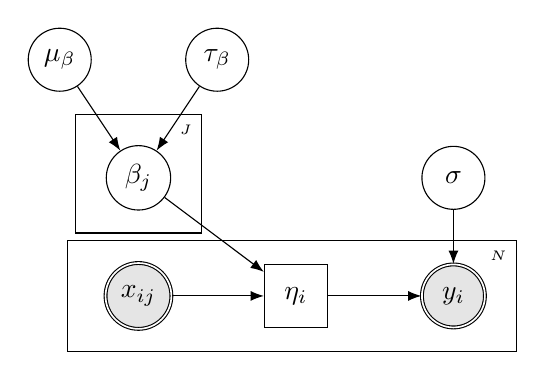
\begin{tikzpicture}[latent/.style={circle, draw, minimum size=8mm}, obs/.style={latent, double, fill=gray!20}, det/.style={latent, rectangle}, >=Latex]
\node[latent] (mu) at (0,3) {$\mu_\beta$};
\node[latent] (tau) at (2,3) {$\tau_\beta$};
\node[latent] (beta) at (1,1.5) {$\beta_j$};
\node[det] (lin) at (3,0) {$\eta_i$};
\node[obs] (x) at (1,0) {$x_{ij}$};
\node[obs] (y) at (5,0) {$y_i$};
\node[latent] (sigma) at (5,1.5) {$\sigma$};
\draw[->] (mu) -- (beta); \draw[->] (tau) -- (beta); \draw[->] (beta) -- (lin); \draw[->] (x) -- (lin); \draw[->] (lin) -- (y); \draw[->] (sigma) -- (y);
\draw (0.2,0.8) rectangle (1.8,2.3) node[below left] {\tiny $J$};
\draw (0.1,-0.7) rectangle (5.8,0.7) node[below left] {\tiny $N$};
\end{tikzpicture}
\end{document}
